\section{Performance test}
This test verifies the performance metrics of the Archive service analyzing different numbers of files, file sizes and archive strategies.

\subsection{Archive performance}
For this test, the an archive process is executed and repeated 4 times to get an average general performance overview. Figure \ref{fig:archivePerformance} illustrates a bar diagram for running an archive process (zipped simulation results) with 7 files, 2 scenarios, 2 result configurations, 2 simulation plans
and 12 simulation runs and results. The results seen in the figure shows that it took about 34.9 s on average to run this process. It is also to be noted that the
simulation results are zipped making their total size about 86 Mb. Figure \ref{fig:archivePerformanceUn} shows the archive process of ths same project without 
compressing the simulation results and it can be seen that the file sizes for the uncompressed process is significantly higher in contrast to the compressed
process with file size on avg about 683 Mb and 43s processing time.

\begin{figure}[H]
    \centering 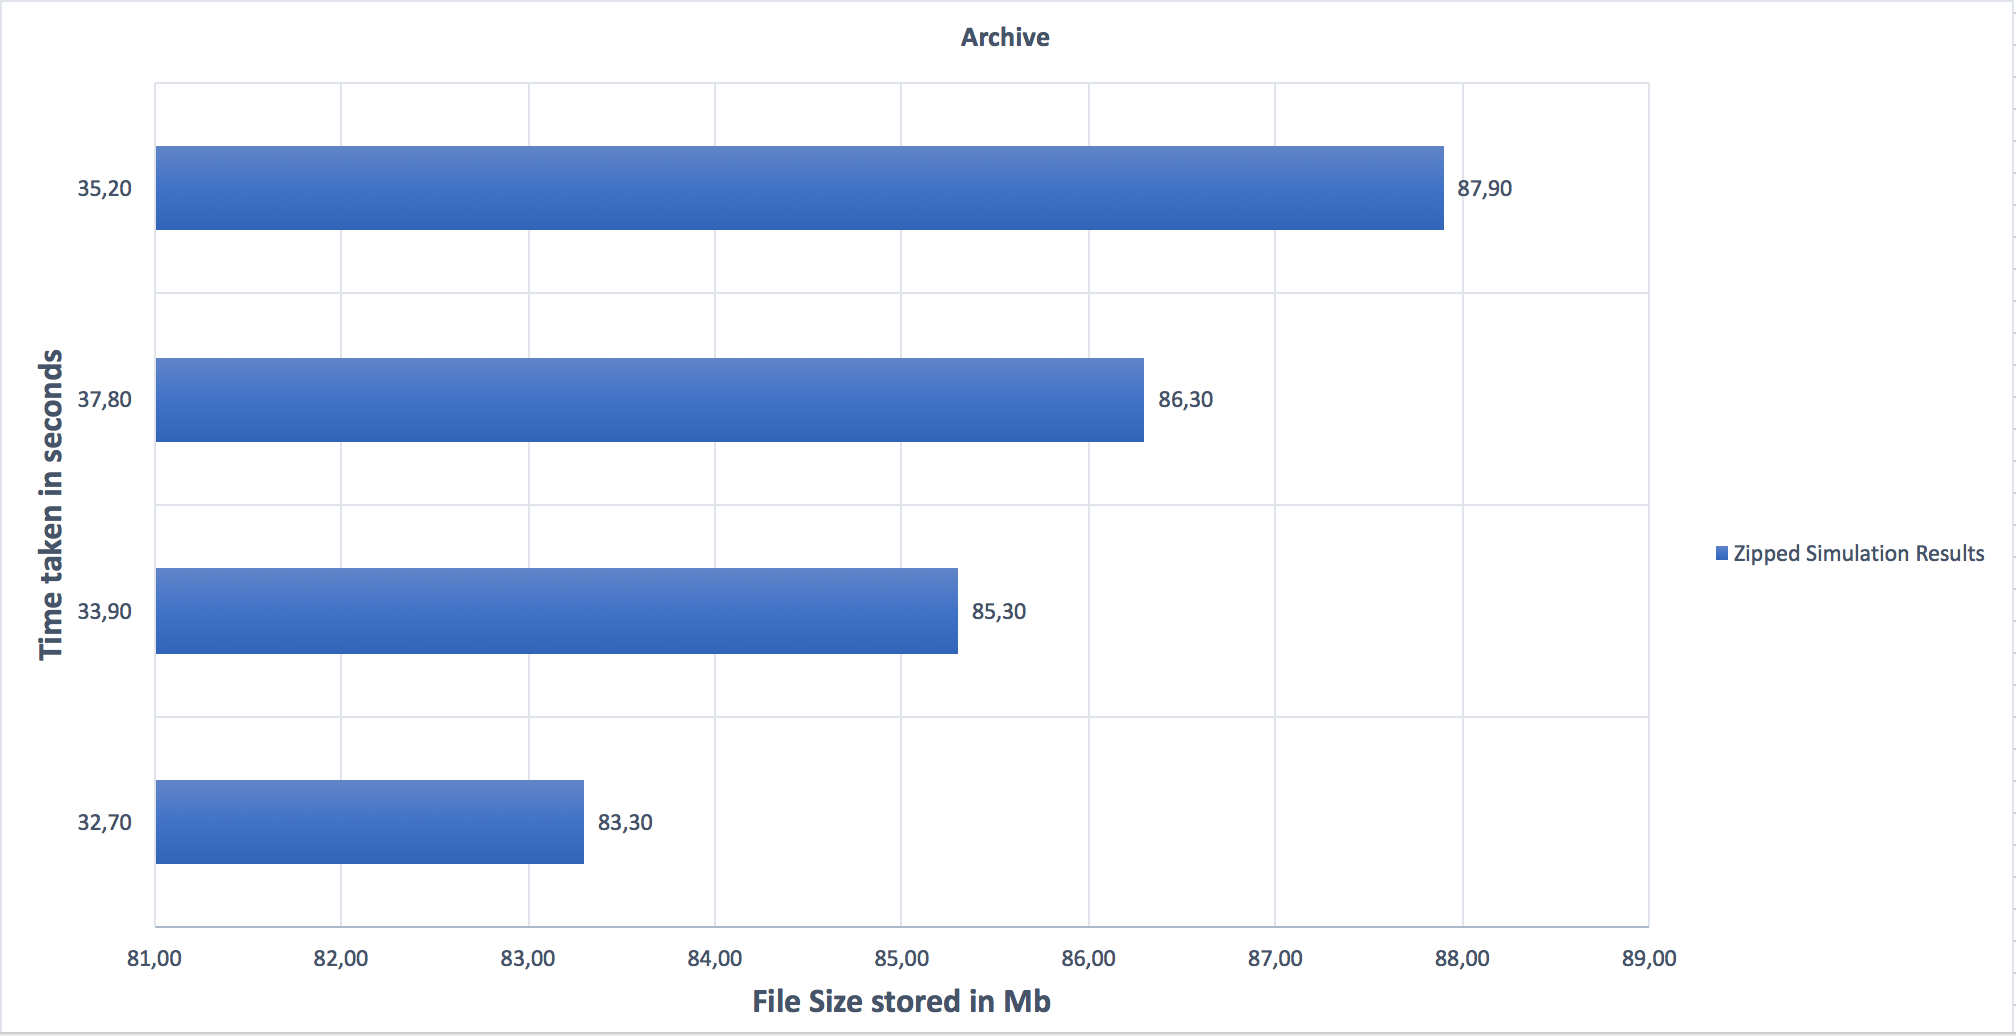
\includegraphics[scale=0.45]{grafiken/archiveZip.png}
    \caption{Overall performance of the archive process (compressed simulation results)}
    \label{fig:archivePerformance}
\end{figure}

\begin{figure}[H]
    \centering 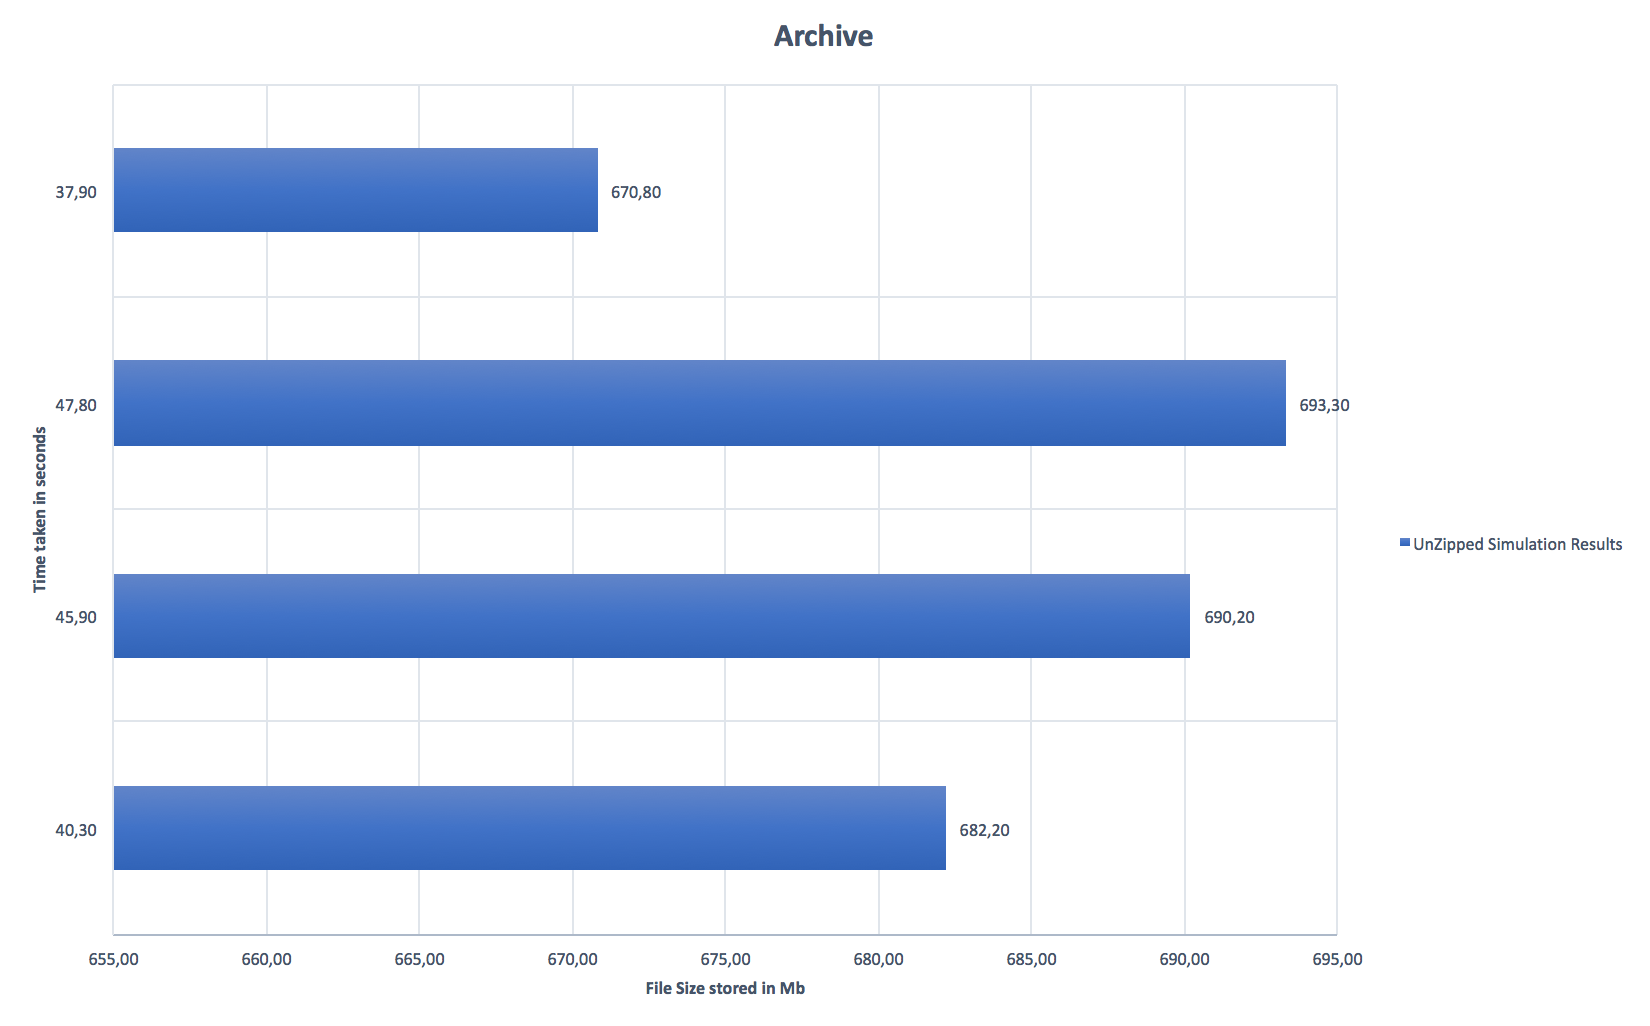
\includegraphics[scale=0.45]{grafiken/archiveUnzip.png}
    \caption{Overall performance of the archive process (uncompressed simulation results)}
    \label{fig:archivePerformanceUn}
\end{figure}

Unfortunately simulation results with larger file sizes could not be tested as no such simulation results was available at the moment but with this metrics it can be said that
for smaller file sizes it is a better choice to compress the simulation data while archiving it since there is a significant data volume save and the time taken for the
archive does not differ by much.   

\subsection{Retrieve performance}
For this test, the same project that was archived is being restored to analyze the performance of the retrieve process. Figure \ref{fig:restorePerformance} illustrates
the results of the retrieve process with the compressed simulation results which takes 4.3 mins on average. Figure \ref{fig:restorePerformanceUn} illustrates the
results of the retrieve process using the uncompressed simulation results which took on average of 4 mins. It is seen that the for projects having their total file
size similar to the analyzed one is benefited by using the compression feature.

\begin{figure}[H]
    \centering 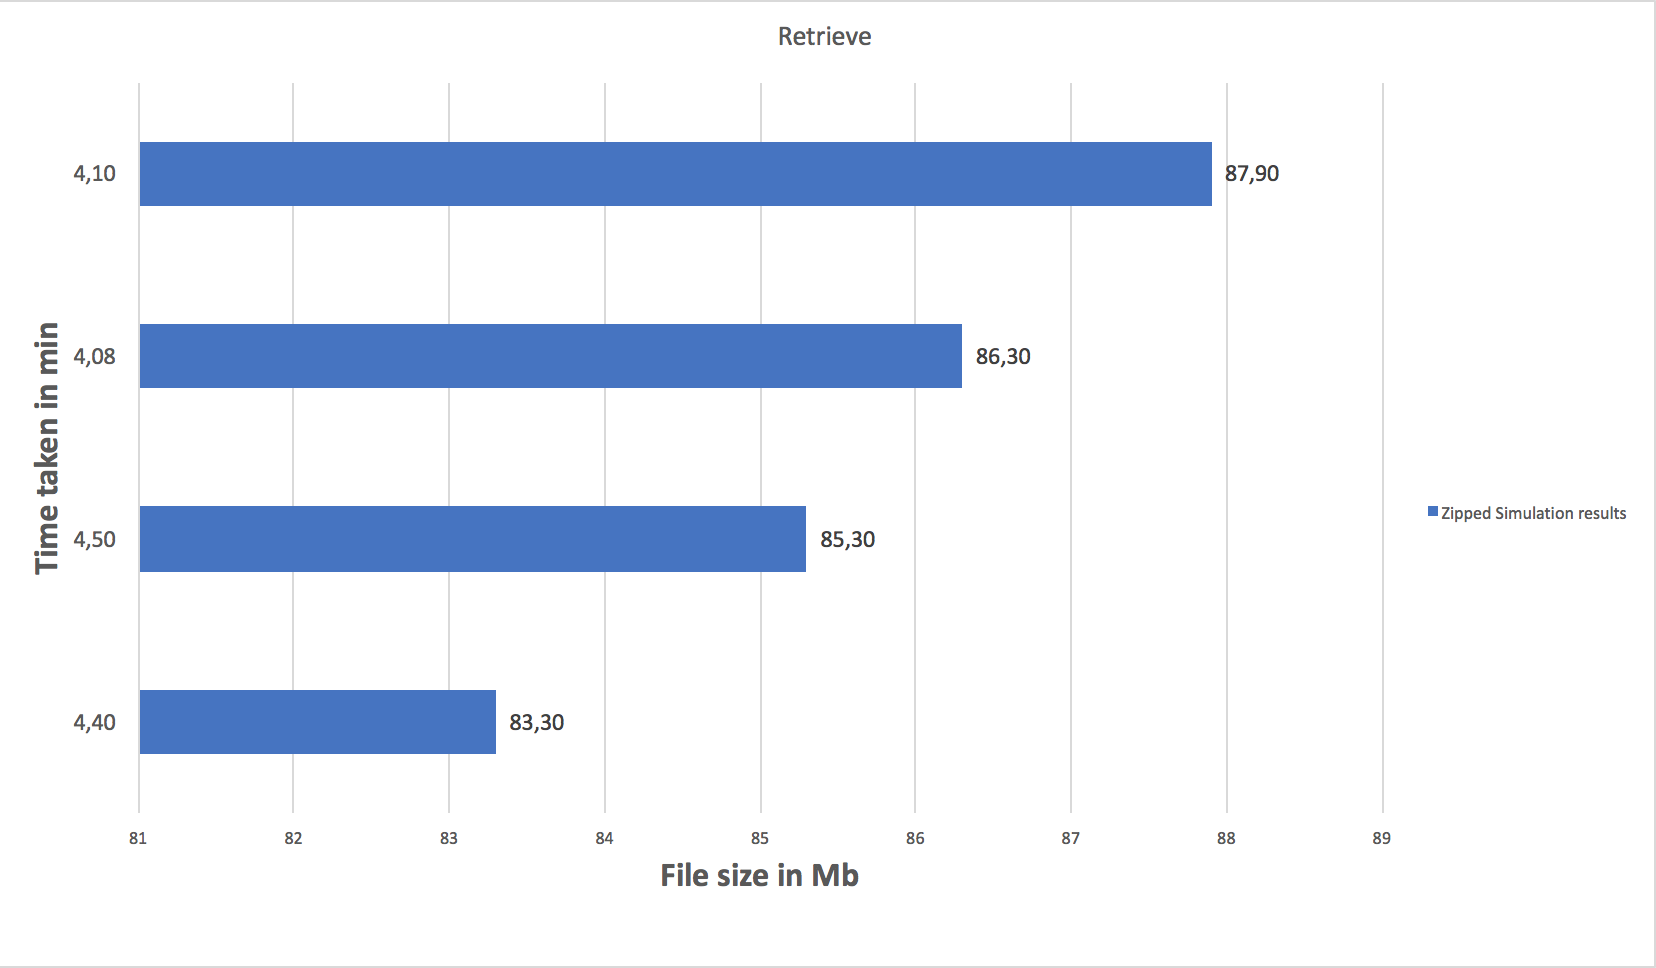
\includegraphics[scale=0.5]{grafiken/retrieveZip.png}
    \caption{Overall performance of the retrieve process (compressed simulation results)}
    \label{fig:restorePerformance}
\end{figure}

\begin{figure}[H]
    \centering 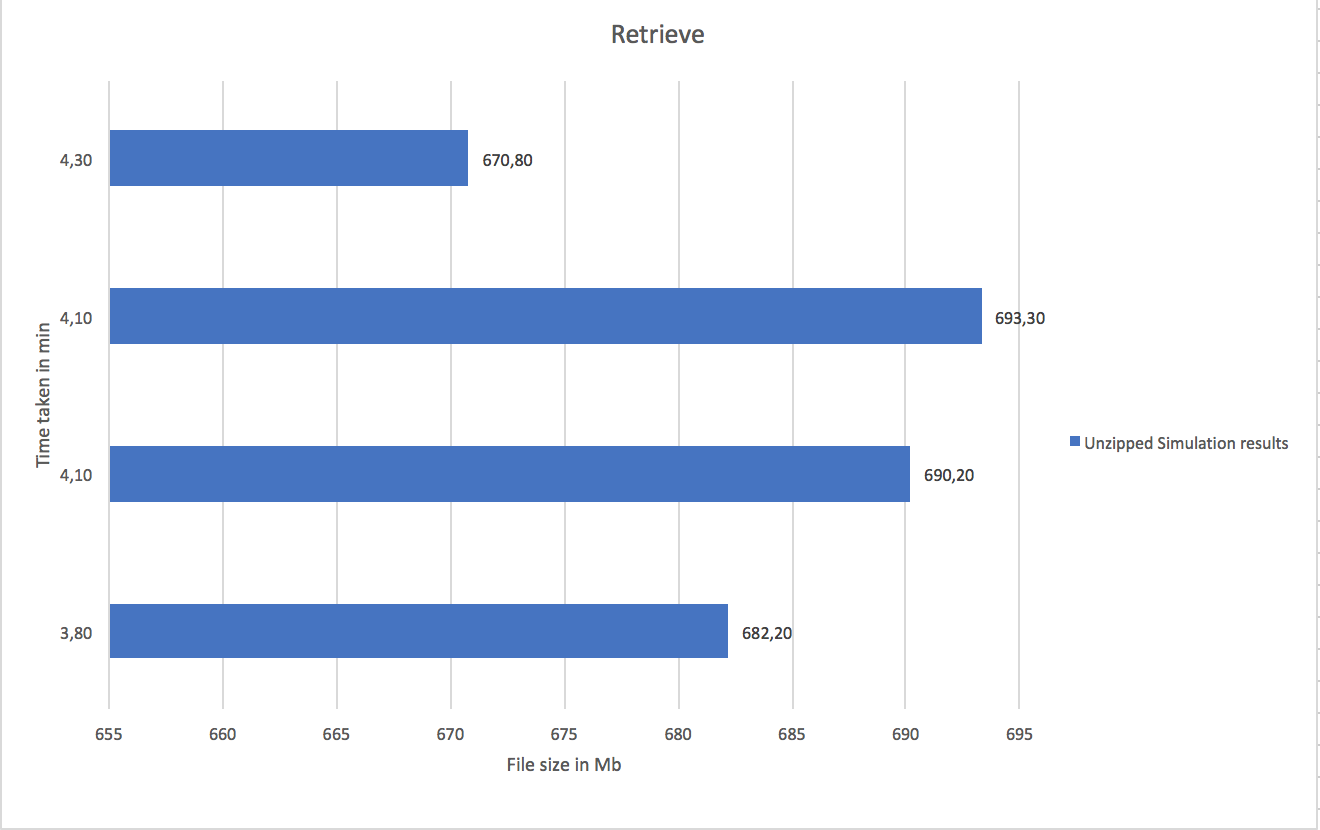
\includegraphics[scale=0.5]{grafiken/retrieveUnzip.png}
    \caption{Overall performance of the retrieve process (uncompressed simulation results)}
    \label{fig:restorePerformanceUn}
\end{figure}

Also, to verify the complexity of the processes the in the same project the number of simulations were doubled i.e. 24 simulation and the performance was recorded
and an average of 55 sec for archive and 8.2 mins for archive was observed. As a result, the processing time was doubled which leads to a
conclusion that the complexity of the algorithm is O(N). It has to be kept in mind that processing time of different kind of models (e.g. KNP, wolves and Sheep) 
would have a different processing time even though the number of files are the same. This is because the processing time are different depending on the complexity of 
the model and the simulation parameters. 